\chapter{Data Aggregatiit With Internal Verification} % (folit
\label{cha:Data Aggregation With Internal Verification}
	
	This chapter describes the rational behind the design specifications of secure aggregation protocol for sensor networks, mechanism used to achieve it and implementation details.
	Then we elaborate the nitty-gritty of the commitment tree generation process with internal verification.

	\section{System Design}

	The most significant design aspect of the sensor network is the \textit{Lifetime of the Network}.
	The sensor network tend to have limited life span as they are powered by the battery.
	The lifetime of the sensor network is inversely proportional to the sensor nodes' power consumption.
	One of the most dominating factor for the power consumption is transmitting and receiving the data between sensor nodes, making network bandwidth an expensive resource.
	The bandwidth is more expensive resource than the local data computation, as trans-receiving activity consumes more power than computation.
	The obvious solution to increase the lifespan of the sensor network is to decrease the bandwidth usage in the network.
	As we know, data aggregation techniques can greatly reduce the bandwidth usage in the network, increasing the lifespan of the network.
	Hence, data-aggregation techniques are one of the key tool in our tool box while designing protocol for the sensor networks.

	The second most significant factor in the design of the data aggregation protocol is \textit{Security Architecture }.
	The International Telecommunications Union (ITU) Telecommunication Standardization Sector (ITU-T) Recommendation X.800, \textit{Security Architect for Open Systems Interconnection} (OSI) provides a systematic approach for it \cite{stallings2008computer}.
	The OSI security architecture focuses on security attacks, mechanism and services defined as follows:\\
	\textbf{Security attack} is any action that compromises the security of information owned by an organization or entity.\\
	\textbf{Security mechanism} is a mechanism that is designed to detect, prevent, or recover from a security attack.\\
	\textbf{Security service} is a service that enhances the security of the data processing systems and the information transfers of an organization.
	The services are intended to counter security attacks, by using one or more security mechanisms.

	\textbf{Security attacks} can be classified as \textit{passive attacks} and \textit{active attacks}.

	\textit{Passive attacks} attempts to learn or make use of information from the system but does not affect the system resources.
	They are in the nature of eavesdropping on, or monitoring of, transmissions.
	Two types of passive attacks are \textit{release of message contents} and \textit{traffic analysis}.

	The \textit{release of message contents} is well understood. 
	A telephone conversation, an electronic mail, and a transferred file may contain sensitive or confidential information.
	We would like to prevent an opponent from learning the contents of these transmissions.

	The \textit{traffic analysis} is subtler. 
	Suppose that we had a way of masking the message so that even if the  opponents captured the message, could not extract it.
	The common mechanism for masking the message is encryption.
	If we had encryption protection in place, an opponent might still be able to observe the pattern of these message communication.
	The opponent could determine the location and identity of communicating hosts and could observe the frequency and length of message being exchanged.
	These patterns might be useful in guessing the nature of the communication that was taking place.

	\textit{Passive attacks} are difficult to detect as they do not involve any alteration of the message.
	Typically, the message traffic is sent and received in an apparently normal way and neither the sender nor receiver is aware that a third party has sniffed the message or observed the traffic pattern.
	However, it is feasible to prevent the success of these attacks, usually by means of encryption. 
	Thus, the emphasis on dealing with passive attacks is on prevention rather that detection.

	\textit{Active attacks} involve some modification of the data stream or the creating of a false stream and can be subdivided into four categories: \textit{replay, masquerade, modification of messages, and denial of service}.

	\textit{Replay} involves the passive capture of a data unit and its subsequent retransmission to produce an unauthorized effect.

	A \textit{masquerade} takes place when one entity pretends to be a different entity.
	For example, authentication sequence can be captured and replayed after a valid authentication sequence has taken place, thus enabling an authorized entity with few privileges to obtain extra privileges by impersonating an entity that has those privileges.

	\textit{Modification of message} means that some portion of a legitimate message is altered or that the messages are delayed or reordered, to produce an unauthorized effect.
	For example, a message stating ``Allow Barack Obama to read confidential file accounts.'' is modified to say ``Allow Michelle Obama to read confidential file accounts.''

	The \textit{denial of service} inhibits the normal use of communication facilities.
	For example, an entity may suppress all messages directed to a particular destination.
	Another form of service denial is the disruption of an entire network, either by disabling the network or by overloading it with messages so as to degrade performances.

	\textit{Active attacks} present the opposite characteristics of passive attacks.
	Whereas passive attacks are difficult to detect, measures are available to prevent their success.
	On the other hand, it is quite difficult to prevent active attacks absolutely, because to do so would require physical protection of all communication facilities and paths at all times.
	Instead, the goal is to detect them and to recover from any disruption or delays caused by them.
	Because the detection has a deterrent effect, it may also contribute to prevention.

	\textbf{Security services} are divided into six categories:
	\textit{Authentication, Access Control, Data Confidentiality, Data Integrity, Non-repudiation, Availability}.

	\textit{Authentication} service assures that a communication is authenticate.
	Two types of authentication services are described in the standard: \textit{peer entity authentication} and \textit{data origin authentication}.

	The \textit{peer entity authentication} provides for the corroboration of the identity of a peer entity in an association.
	Two entities are considered as peer if they implement the same protocol in different systems (e.g., two TCP users in two communicating systems).
	Peer entity authentication is used at the establishment of, or at times during the data transfer phase of, a connection.
	It attempts to provide confidence that an entity is not performing either a masquerade or an unauthorized replay of a previous connection.

	\textit{Data origin authentication} provides the corroboration of the source of a data unit. 
	It does not provide protection against the duplication or modification of data units.
	This type of service supports applications like electronic mail where there are no prior interactions between the communicating entities.

	\textit{Data Confidentiality} ensures the protection of transmitted data from passive attacks.
	It is also known as secrecy or privacy.
	For example, student grade information is an asset whose confidentiality is considered to be highly important by students.
	In the United States, the release of such information is regulated by the Family Educational Rights and Privacy Act (FERPA).
	Grade information should only be available to students, their parents, and employees that require the information to do their job.
	The other aspect of confidentiality is the protection of traffic flow from analysis.
	This requires that an attacker not be able to observe the source and destination, frequency, length, or other characteristics of the traffic on a communications facility.
	Ensuring confidentiality can be difficult.
	For example, who determines which parties are authorized to access the information?
	By ``accessing'' information, do we mean that an authorized party can access a single bit? the whole collection? pieces of information out of context?
	Can someone who is authorized disclose that information to other parties?\cite{pfleeger2002security}

	\textit{Data Integrity} assures that the only authorized entities can modify the information; where modification means writing, creating, deleting and changing the information.
	A hospital patient's allergy information stored in a database illustrates the several aspects of the data integrity.
	The doctor should be able to trust that the information is correct and current.
	Now, suppose a nurse who is authorized to view and update the information deliberately falsifies the data to cause harm to the hospital.
	The database needs to be restored to a trusted basis quickly, and it should be possible to trace the error back to the person responsible.
	Patient allergy information is an example of an asset with a high requirement for integrity. 
	Inaccurate information could result in serious harm or death to a patient and expose the hospital to massive liability.
	Because the integrity service relates to active attacks, we are concerned with detection rather than prevention.
	If a violation of integrity is detected, then the service may simply report this violation, and some other portion of software or human intervention is required to recover from the violation.
	Alternatively, there are mechanisms available to recover from the loss of integrity of data, as we will review subsequently. The incorporation of automated recovery mechanisms is, in general, the more attractive alternative.

	\textit{Availability} means that the information of a system being accessible and usable by an authorized parties according to performance specification at appropriate times.
	In other words, if some person or system has legitimate access to a particular set of objects, that access should not be prevented.
	Availability applies to the information and services.
	For example, information or service is available can mean the following. 
	It is present in the usable form, having the enough capacity to meet the service need.
	If it is in wait mode, it is making enough progress, and it has a bounded waiting time, meaning there is timely response to our requests.
	Resources are allocated fairly so that some requests are not favored over the others.
	The service can be used easily and in its intended way.
	Availability addresses the concern raised by the denial of service attacks.
	It depends on proper management and control of system resources and thus depends on access control service and other security services.

	\textit{Non repudiation} service requires neither the sender nor the receiver can deny the transmission.
	Thus, when a message is sent, the receiver can prove that the alleged sender in fact sent the message.
	Similarly, when a message is received, the sender can prove that the alleged receiver in fact received the message.
	This is very important in electronic commerce applications, where it is important that a consumer cannot deny the authorization of a purchase.

	\textit{Access Control} is the ability to restrict and control the access to host systems and applications via communications links.
	To achieve this, each entity trying to gain access must first be identified, or
	authenticated, so that access rights can be tailored to the individual.
	Login credentials and Locks are two analogues mechanism of access control.

	\textbf{Security mechanisms} follow one of the most fundamental principle of Open Design \cite{bishop2004introduction} defined as follows:
		\begin{definition}
			The principle of open design states that the security of a mechanism should not depend on the secrecy of its design or implementation.
			\label{def:open-design}
		\end{definition}
		Designers and implementers of a program must not depend on secrecy of the details of their design and implementation to ensure security.
		Others can ferret out such details either through technical means, such as disassembly and analysis, or through nontechnical means, such as searching through garbage receptacles for source code listings (called ``dumpster-diving'').
		If the strength of the program's security depends on the ignorance of the user, a knowledgeable user can defeat that security mechanism.
		The term ``security through obscurity'' captures this concept exactly.
		This is true of cryptographic software and systems.
		Because cryptography is a highly mathematical subject, and companies who sell these softwares want to keep their algorithms secret. 
		Issues of proprietary software and trade secrets complicate the application of this principle.
		In some cases, companies may not want their designs made public, lest their competitors use them.
		The principle then requires that the design and implementation be available to people barred from disclosing tit outside the company.
		Note that keeping cryptographic keys and passwords does not violate this principle, because a key is not an algorithm.
		However, keeping the enciphering and deciphering algorithms secret would violate it.
		The following security mechanisms may be incorporated into the appropriate protocol layer in order to provide some of the OSI services.

		\textit{Encryption} is the use of mathematical algorithms to transform data into a form that is not readily intelligible.
		The transformation and subsequent recovery of the data depend on an algorithm and zero or more encryption.

		\textit{Digital Signature} appends the data to a cryptographic transformation of data unit that allows a recipient of the data unit to prove the source and integrity of the data unit and protects against the forgery (e.g., by the recipient).

		\textit{Traffic Padding} is the insertion of bits into gaps in a data stream to frustrate traffic analysis attempts.

		\textit{Routing Control} enables selection of particular physically secure routes for certain data and allows routing changes, especially when a breach of security is suspected.

		\textit{Notarization} is the use of a trusted third party to assure certain properties of a data exchange.

		\textit{Authentication Exchange} is a mechanism intended to ensure the identity of an entity by means of information exchange.

		\textit{Hash functions} provides one way functions to achieve irreversible encryption.

	As you can see, expectations from secure networking protocol are far-reaching.
	It is very ambitious for any system to have all the above mentioned security services at the same time.
	If we have to achieve all the security services for sensor networks we can make each sensor node signs its reading data and then send data with its signature to its parent.
	And the network forwards all the data with their respective signatures to the base station.
	The base station verifies all the signatures and then calculates the aggregate function.
	Clearly, this approach is not practical as it requires $n$ signatures to traverse through the link between the base station and the root node of the network; where $n$ is the number of nodes in the network.
	Which makes that link the bottleneck link of the network. 
	And if that link breaks we loose the entire network connectivity.

	In reality all the security services are not always required.
	For an instance, when a client downloads a file from the File server using Internet, he can verify the integrity of the File using the checksum.
	But it is okay if somebody on the network sniffed the downloading activity as far as it did not change the content of the File.
	In this application, a client requires the integrity of the File but the privacy of the client, the File server and the Internet service provider are not required.
	To give an analogy with a physical world application, when a person writes a postcard, he puts his own signature on the it. 
	When that postcard delivers successfully by the postal service, the receiving party can verify the integrity of the message from the handwriting and the signature of the person.
	The postal service knows the sender and the receiver of the postcard.
	It can even read the postcard.
	Again, here integrity is important not the confidentiality.
	It is crucial to find out which security services are desired for the particular application, so we can use the relevant security mechanisms to provide those services.
	In practice, protocol designer finds out the most important security services for the applications before designing the protocol.

	For example, Wagner's work \cite{wagner2004resilient} describes the attacks on standard schemes for data aggregation and introduces the problem of securing aggregation in the presence of malicious or spoofed data.
	He proposes a mathematical theory of security for aggregation.
	The theory quantifies, in a principled way, the robustness of an aggregation operator against malicious data.
	It draws novel connections to statistical estimation theory and to the field of robust statistics.
	He identifies techniques for aggregation that provide robustness against attack. 
	It provides helpful guidance to sensor network implementors or designers in selecting appropriate aggregate functions.

	Secure Information Aggregation (SIA) \cite{przydatek2003sia}  address the problem of how to enable secure information aggregation, such that the user accepts the data with high probability if the aggregated result is within a desired bound, but that the user detects cheating with high probability and rejects the result if it is outside of the bound.
	SIA provides statistical security under the assumption of a single-aggregator model.
	In the single-aggregator model, sensor nodes send their data to a single
	aggregator node, which computes the aggregate and sends it to the
	base station.
	This form of aggregation reduces communications only on the link between the aggregator and the base station, and is not scalable to large multihop sensor deployments.
	SIA provides the probabilistic data-integrity service under strong network assumptions.

	Secure Hierarchical In-network Aggregation (SHIA) \cite{chan2006secure}, in many ways enhances Secure Information Aggregation (SIA).
	SHIA presents the provably secure sensor network data aggregation protocol for general networks and multiple adversarial nodes, in compare to SIA which provides probabilistic security for a single aggregate network topology.
	SHIA limits the adversary’s ability to manipulate the aggregation result with the tightest bound possible, with no knowledge of the distribution of sensor data values.
	SHIA provides data-integrity service for any hierarchical sensor networks because of that it can detect malicious activity in the network.

	The third most significant aspect in the design of secure data aggregation protocol is \textit{Data Integrity}.
	The protocol collects the data from the sensors and aggregates the reading on the way to the base station.
	The base station takes an important decision based on the received value.
	For example, if the sensor network is deployed to measure the certain harmful chemical levels in the lab atmosphere and raise an alarm if the it increases above certain level.
	And if the base station fails to raise an alarm because of the false aggregated data, can create catastrophic and lethal situation.
	Hence, the data integrity is so important.

	As we know, data integrity can be achieved with the error detection and error correction techniques.
	The first step towards achieving the data integrity in the sensor network is to \textit{detect any malicious activity} in the network.
	And the second step is the ability to \textit{locate the malicious node or an adversary} in the network.
	We think detecting a malicious activity without tracing down the malicious node responsible for it, is of no value.
	To give an analogy with the physical world, it is like you know there is a crime in the city and you do not do anything about it.
	Locating the criminals responsible for the crime is mandatory to abolish the crime in the city.
	In similar way, locating the malicious node and removing it from the network is an important security service. 
	Failing to provide such a security service, allows an adversary to continue doing the malicious activity in the future, which makes aggregated sensor data garbage. 
	And network has to redo the all the work to create response for the query from the base station, which consumes lots of bandwidth. 
	An adversary can repeat this process until the network dies due to low battery power, creating a denial of service attack in the network.
	Hence, we think detecting a malicious node who is responsible for the malicious activity is equally important.
	If we can track down the malicious node in the network then we can remove that node from the network for all future queries.
	And make sure that all the future queries are not manipulated by any malicious node in the network.
	Hence, the fourth and fifth most significant design aspects of secure aggregation protocol are \textit{detect the malicious activity} (in terms of data aggregation) and can \textit{detect the adversary} in the network, respectively.

	To detect an adversary (or prove someone guilty), we need proof that the adversary is responsible for the malicious activity.	 
	% To achieve our goal, we think the Digital signature is the perfect cryptographic tool.
	Consider the following example showing the analogy with the signature scheme in the physical world, used by the postal services.
	When a postman delivers the package, the receiving party has to sign the document informing that he verified and received the package.
	As only the receiving party can create his signature, in the future he can not claim of not receiving the package or receiving the damaged or incorrect package. 
	And if he claims such, the postal company has the signed document as the proof mentioning that the package was received successfully, by the receiving party.
	The signed document also ensures to the postal company that the postman did not misplace or steal the package.
	The signature scheme used by the postal service promises 
	% authenticity (assures the origin of the message) and 
	non repudiation security service.
	Hence, we require \textit{non-repudiation} security service in the sensor network.

	% With Digital signatures one can achieve \textbf{non-deniability  (non repudiation), authentication, integrity} (assures that only the authorized parties can modify the message) as described in Section \ref{sec:digital-signature}.

\section{System Design Specifications}
	We want to design a secure aggregation protocol which maximizes the \textit{network lifetime}.
	The protocol can be applied to \textit{any hierarchical sensor network}.
	We want protocol to work on \textit{resilient} and \textit{non-resilient} aggregate functions without compromising any desired security properties.
	We want protocol to be secure with \textit{a single} or \textit{multiple adversaries} in the network.
	\label{subsec:security benefits of signing the data-item}	We want the protocol to protect against any \textit{active attacks}. 
	If the aggregation result is accepted by the base station it should have very high confidence in the result, meaning that we want the highest level of \textit{data integrity} security service in the protocol.
	We want the capabilities to \textit{detect any malicious activity}.
	If there is any malicious activity in the network, we should be able to \textit{locate an adversary} responsible for it, in the network.
	We want the \textit{non-repudiation} security service so neither sender nor receiver can deny the transmission or receiving of the message, which is mandatory to locate an adversary.
	We want to achieve this with the least amount of \textit{bandwidth and computation} overhead in the network.
	So, the protocol can be easily implemented in the real world sensor networks.
	It is not that difficult to provide mentioned security properties to protect against active attacks in the sensor network. 
	We will show that it requires sub-linear edge congestion to provide these services. 
	% As we saw in the previous chapter SHIA can detect the malicious activity in the network with only sub-linear edge congestion.
	% So, we built our work on top of SHIA which can detect an adversary.


	% For that we want non-repudiation

	% If there is any malicious activity detect it

	% Locate an adversary	
	% fig:Commitment payload of C to detect an adversary in the network with least amount of overhead in terms of BW and computation.
	% We wanted to achieve that with as realistic as possible. 


% \section{Design Goals}


% 	% In the previous chapter, we saw that SHIA limits the adversary's ability to manipulate the aggregation result with the tightest bound possible.
% 	% But, SHIA uses truncated sum as an aggregate function which is resilient according to the Wagner \cite{wagner2004resilient}.
% 	% It does not help accurately calculating the sum aggregate. 
% 	% Furthermore, SHIA does not help detecting and revoking the from the of Sensor Node malicious aggregate no network.
% 	% SHIA does not require prior knowledge of network topology and works on hierarchical sensor network which might include multiple malicious sensor nodes, with only suboptimal congestion overhead.
% 	% SHIA helps the sensor node verify, its reported sensor reading was aggregated correctly or not, by an an aggregate node.
% 	% If an an aggregate node has tampered with the reported sensor reading then the relevant sensor node can detect the tampering and raise an alarm.
% 	We develop the aggregation protocol which works for any random hierarchical sensor networks with a single or multiple adversaries.
% 	It works on the resilient as well as non-resilient aggregation functions Defined in \ref{def:resilient}, without compromising any desired security properties.
% 	It
% 	It prevents masquerade attacks in the network so this protocol can easily be applied to do the voting scheme in the network.

	% We want to achieve all the mentioned goals by inducing only $O(\delta \log^{k} n)$ node congestion in the aggregation tree; where $n$ is the number of nodes in the network, $\delta$ is the fanout of any node in the aggregation tree, and $k$ is the variable.
	% Ideally, we want $k=0$, in the case of SHIA and our protocol $k=2$, which will be explained in the later chapter.
	% % which is built on top of commitment tree generation of SHIA mentioned in the previous chapter.

\section{Security Mechanisms}
	To detect any malicious activity in the network which is an important part of achieving data-integrity in the network we use \textit{Hash Functions} as security mechanism.
	To protect against any active security attacks, provide authentication and non-repudiation security services we use \textit{Digital Signatures} as the security mechanisms.
	Both of these mechanisms are described in details in Chapter \ref{cha:Networking and Cryptography tools}.	


\section{System Design Implementations}
	The high level idea of the aggregate commit with verification scheme is that all the nodes in the network send the signature of the message along with the message itself. 
	It sends its certificate if the parent node does not have it already.
	The parent node verifies all the received signatures from its children.
	And proceeds with the aggregation process.
	After aggregation, the parent node can throw away all the signatures from its children and signs the message of its children or it can pass its children's signatures to its parent. 
	The pros and cons of each approach are discussed in the following sections. 

\section{Data-Item}
	
	We describe structure of the data-item, used in creating the commitment tree for the aggregate commit with verification approach. And differences between the data-item and the label structure of SHIA, with rational behind it.
	\begin{definition}
		\label{def:data-item}
		A commitment tree is a binary tree where each vertex has an associated data-item representing the data that is passed on to its parent. The data-items have the following format:

		$\hspace{100pt}$ \textbf{$<\ $id, count, value, commitment$\ >$}\\
	Where $id$ is the unique ID of the node; $count$ is the number of leaf vertices in the subtree rooted at this vertex; $value$ is the SUM aggregate computed over all the leaves in the subtree and $commitment$ is a cryptographic commitment.
	\end{definition}
	
	We remove the $complement$ field from the label structure Defined \ref{def:label}. 
	We think the complement filed is redundant information in the label. 
	The complement field is used by the base station (the querier, according to SHIA), before the result checking phase, to verify \textbf{SUM + COMPLEMENT =} $\textbf{n} \cdot \textbf{r}$ ; where $\textbf{n}$ is the number of nodes in the network, $\textbf{r}$ is the upper bound on the allowed sensor readings.
	We can achieve the same upper bound without the complement field.
	As the querier knows $n, r$ and it gets SUM from the root of the aggregation tree.
	If \textbf{SUM} $> \textbf{n} \cdot \textbf{r}$ , then the base station knows some node or nodes in the network reported out of range readings.

	We include $id$ of the node in its data-item.
	SHIA does not have the ID field in their label structure as they do not do internal verification while creating a commitment tree and while distributing off-path values.
	Also, in the label format ID of the node is hashed in the commitment field after the first aggregation and virtually gets lost.
	Hence, SHIA can not provide security services such as authenticity, non-repudiation and is vulnerable to all sorts of active attacks.
	We do internal verification while creating the commitment tree and distributing off-path values.
	So, it is necessary for any aggregate node to know the ID of all the received data-items in its forest, for the verification of the received signatures as shown in the next section.

\section{Signing the Data-Item}
	During commitment tree generation phase, there is one vertex $S_{0}$ for each sensor node $S$, which we call the leaf vertex of $S$.
	The data-item for leaf vertex $S_{0}$ and associated signature to it is defined as follows:
	\begin{equation}
		\label{eq:leaf-vertex}
		S_{0}\ =\ <S_{id}, 1, S_{value}, H(N||1||S_{value})>;\ 	\textsf{Sign}_{S_{S}}(S_{0})
	\end{equation}
	where $H$ is a collision resistant hash function, $S_{S}$ is the secret key of sensor node $S$, $N$ is the query nonce.

	The key difference between the SHIA's approach and our approach is that, in addition to sending the data-item, each sensor node sends the signature of the data-item to its parent.
	It sends its certificate as well if the parent node does not have it in its memory  already.
	The parent node gets the public key of the child node from its certificate, which is used in verifying the signature. 
	The parent node verifies all the received signature using its children node's public key.
	Details of the signing and verification processes are shown in Figure \ref{fig:digita-signature}.
	After doing the verification the parent node proceeds to the aggregation and creating the commitment tree.
	
	\subsection{Bandwidth Analysis}

	Cite resources for this.
	
	Typical size of the data-item packet is $400$ bits.
	If one uses Elliptic curve cryptography then the size of signature is $500$ bits.
	And the certificate size is $1500$ bits.
	So, at max we have to send additional $2000$ bits with the data-item.
	We think it is worthwhile to send these additional bits.
	Because of all the security benefits we gain from it. 
	\textbf{Note:} The packets size are close approximate to the actual packet size. 
	The actual packet size may differ based on the implementation.

	\subsection{Security Benefits}
	\label{subsec:security benefits of signing the data-item}
	The signature allows the parent node to verify the \textit{authenticity} of the sensor node.
	It also allows to verify the \textit{integrity} of the received data-item.
	It allows the sender to have the proof for the sent data-item.
	And the receiver for the proof for the received data-item, providing the \textit{non-repudiation}.
	Hence, it protects against the \textit{active attacks}.

\section{Signing the Commitment Payload}
		We define commitment payload based on the commitment forest Defined in \ref{def:commitment-forest}.
	\begin{definition}
		A \textbf{commitment payload} is a set of data-items of the root vertices of the trees in the outgoing commitment forest.
	\end{definition}
	% We use the term payload for commitment payload and the term forest for the commitment forest.
	For brevity, we use the term forest, payload instead of commitment forest, commitment payload respectively.

	An aggregate node sends an additional signature to its parent, which is a signature of all the data-items in its payload.
	The signature on the payload assures that an aggregate node sent only the data-items included in the payload signature.
	It assures the authenticity, non-repudiation, integrity of all the data-items included in the payload.
	For example, the aggregation tree shown in Figure \ref{fig:Palm aggregation tree}, the payload of sensor node $C$ is show in Figure \ref{fig:Commitment payload of C}.
			\begin{figure}[h!]
				\centering
				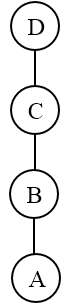
\includegraphics[scale = 1]{images/palm-aggregation-tree.png}\\
				\caption{Palm Shaped Aggregation Tree}
				\label{fig:Palm aggregation tree}
			\end{figure}
		The sensor node $C$ sends all the data-items in its payload with their signatures to its parent sensor node $D$.
		Furthermore, $C$ sends the signature of its payload $\textsf{Sign}_{S_{C}}(C_{0}||B_{1})$ to $D$.\\
			\begin{figure}[h!]
				\centering
				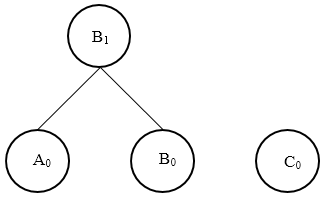
\includegraphics[scale = 1]{images/commitment-payload-of-C.png}
				\caption{Commitment Payload of Sensor Node $C$}
				\label{fig:Commitment payload of C}
			\end{figure}
		\begin{equation}	
			\begin{array}{l}
				B_{1} =\ <B_{id}, 2, B_{1value}, H(N||2||B_{1value}||A_{0}||B_{0})>;\ \textsf{Sign}_{S_{B}}(B_{1})\\
				C_{0} =\ <C_{id}, 1, C_{value}, H(N||1||C_{value})>;\ \textsf{Sign}_{S_{C}}(C_{0})\\
				\textcolor{red}{\textsf{Sign}_{S_{C}}(C_{0}||B_{1})}
			\end{array}
			\label{eq:forwarding-payload-without-resigning}
		\end{equation}

	\subsection{Security Benefits}
	In addition to all the security benefits mentioned in Subsection \ref{subsec:security benefits of signing the data-item}, signature on the $C$'s payload $\textsf{Sign}_{S_{C}}(C_{0}||B_{1})$ assures that the sensor node $C$ sent only two data-items $C_{0},B_{1}$ in its payload.
	And none of the data-items in its payload have been left stranded.

\section{Forwarding the Commitment Payload}	
	% This example showcases another important aspect of the protocol.
	% It shows two different ways of creating a commitment tree.
	The sensor node $C$ has two data-items $C_{0},B_{1}$ in its payload as shown in Equation \ref{eq:forwarding-payload-without-resigning}. 
	It sends the $\textsf{Sign}_{S_{B}}(B_{1})$, $\textsf{Sign}_{S_{C}}(C_{0}) $ and $\textsf{Sign}_{S_{C}}(C_{0}||B_{1})$ to its parent node $D$.
	It requires the parent node $D$ to know the public key of the sensor nodes $C$ and $D$, hence their certificates.
	Instead of that the sensor node $C$ can verify the $\textsf{Sign}_{S_{B}}(B_{1})$ then remove the old signature and create new signature $\textsf{Sign}_{S_{C}}(B_{1})$ signed by itself on the data-item $B_{1}$ as shown below:
\begin{equation}	
	\begin{array}{l}
		B_{1} =\ <B_{id}, 2, B_{1value}, H(N||2||B_{1value}||A_{0}||B_{0})>;\  \textcolor{red}{\textsf{Sign}_{S_{C}}(B_{1})}\\
		C_{0} =\ <C_{id}, 1, C_{value}, H(N||1||C_{value})>;\ \textsf{Sign}_{S_{C}}(C_{0})\\
		\textsf{Sign}_{S_{C}}(C_{0}||B_{1})
	\end{array}
	\label{eq:forwarding-payload-with-resigning}
\end{equation}
We call these two approaches \textbf{Forwarding signatures without resigning the data-items}, \textbf{Forwarding signatures with resigning the data-items} as shown in Equations \ref{eq:forwarding-payload-without-resigning} and \ref{eq:forwarding-payload-with-resigning} respectively .

To give an analogy with the real world application consider the following example.
One want to buy a diamond from the local diamond retailer.
Diamond is an expensive commodity so the end customer wants to verify its authenticity and integrity before purchasing.
Suppose, the diamond was created by the manufacturer in Africa, it was sold to a national wholesaler in the United States. 
The national wholesaler sells it to the state level reseller and he sells it to the city or county level retailer from whom the customer purchases the diamond.

One approach to verify the authenticity of the commodity is to make each entity in the supply chain to verify all the signatures on the received entity and sign on top of it.
And then forward the commodity with all the signatures to the next entity in the supply chain.
The next entity repeats the same procedure.
Hence, any entity in the supply chain need to verify the signatures of all its descendants in the supply chain.
In our example, it means to make the manufacturer from Africa signs the diamond and sells the signed diamond with his certificate to the national level wholesaler in United States.
The national level wholesaler in United States verifies the signature from the manufacturer using manufacturer's certificate.
Then he adds his signature and certificate, and sells the diamond signed with two signatures and two certificates to the state level reseller.
The state level reseller verifies both the signatures on the diamond using the respective certificates.
Then he adds his signature and certificate, and sells the diamond singed with three signatures and three certificates to the city level retailer. 
The city level retailer does the same thing before selling the diamond to the end customer.
In the end, the customer needs to verify all four signatures, using the respective certificates.

% Note: that the same diamond now has been signed by four different entities. And the end customer need to know the certificate of all four parties to verify all those signatures.

An alternative approach to verify the authenticity of the commodity is to make each entity in the supply chain verify the signature, throw away the old signature, and then add its own signature on it. 
It means the next entity in the supply chain need to verify only a single signature.
The next entity repeats the same procedure.
Hence, any entity in the supply chain need to verify the signature of only its direct peer in the supply chain. 
In our example, it means to make the manufacturer from Africa signs the diamond and sells the signed diamond with his certificate to the national level wholesaler in United States.
The national level wholesaler in United States verifies the signature from the manufacturer using the manufacturer's certificate.
Then he removes the signature of the manufacturer, adds his own signature and certificate, and sells the diamond signed with one signature and one certificate to the state level reseller.
The state level reseller verifies only the signature from the wholesaler using the wholesaler's certificate.
Then he removes the signature of the wholesaler, adds his own signature and certificate, and sells the diamond signed with one signature and one certificate to the city level retailer.
The city level retailer does the same thing before selling the diamond to the end customer.
In the end, the customer needs to verify only one signature of the city level retailer using retailer's certificate.
This approach requires very few number of certificates overall in the supply chain.

Both theapproaches have their pros and cons and the perfect approach depends heavily on the application.
The various aspects of both the approaches for sensor nodes are discussed in the following sections.

	\section{\textcolor{red}{Forwarding signatures with resigning the data-items}}
		If we throw away the old signatures and resign the data-item with current aggregate node then following is true:
			\begin{itemize}
				\item Each parent needs the certificates of only its direct children.
				\item Each child needs to know the certificate of its parent only.
				\item Number of signatures remain the same as previous approach.
				\item Number of certificates needed in the network is $O(n)$; n is the number of nodes in the network.
				\item We do not need the signature of the payload.
			\end{itemize}
		As the commitment tree is binary we need $\Omega(2^h - 1)$ signatures; where $h$ is the height of the commitment tree in both approaches .
		% Analysis model:	
		% 	While creating CT;While distributing off-path; Both places together\\
		% Initial analysis says, if a single aggregate node cheats while CT generation or distributing off-path values it gets caught.
			\begin{table}[!htb]	
		\begin{center}
			\begin{tabular}{ |l| l| l| }
		    \hline
		    & With resigning & Without resigning \\
		    \hline
		    Number of signatures & Test & T \\	
		    \hline
		    Number of signing activity & Test & T \\
		    \hline
		    Number of verifying activity & Test & T \\
		    \hline
		    Number of certificates & Test & T \\
		    \hline
			\end{tabular}
		\end{center}
		 \caption{System-on-Chip specifications for IEEE 802.15.4 from TexasInstruments}
		 \label{table:soc}
	\end{table} 
		Note that we send signatures while distributing off-path values.
	\section{\textcolor{red}{Forwarding signatures without resigning the data-items}}

	\section{Commitment Tree Generation}
	For the given aggregation tree the commitment forest is built as follows.
	Leaf sensor nodes in the aggregation tree create their leaf vertex by creating data-items and their respective signatures according to Equation \ref{eq:leaf-vertex}, \ref{eq:signature-leaf-vertex} which they send it to their parent as a payload in the aggregation tree.
	Each internal sensor node $I$\ in the aggregation tree also creates their leaf vertex and its signature.
	In addition, $I$\ receives the payload from each of its children which creates the forest for $I$.
	Once $I$ verifies all the received signatures, it merges all the data-items in its forest with same count value to create its payload.
	Note that we can determine the height of the commitment tree from the count value.

	Suppose $I$ have to create its payload by merging $i$ data-items $D_{1}$, $D_{2}$, $\dotsc$, $D_{i}$ in its forest.
	First, $I$ verifies the received signatures $Sign(D_{1})$, $Sign(D_{2})$, $\dotsc$, $Sign(D_{i})$.
	Once verified, $I$ starts merging the data-items as follows.
	Let $c$ be the smallest count value in $I$'s forest.
	The sensor node $I$ finds two data-items $D_{1},D_{2}$ in its forest with the same count value $c$ and merges them into a new data-item with the count of $c+1$ as shown in Figure \ref{fig:increase-height}.
	\begin{figure}[h!]
		% \centering
		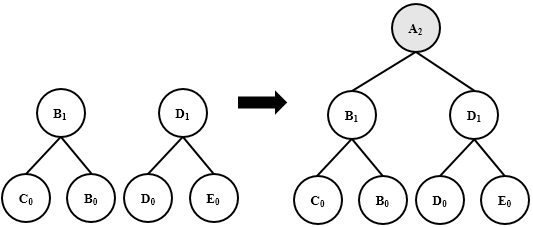
\includegraphics[width=6in]{images/increase-height.png}\\
		\caption{$A$ has $B_{1}, C_{1}$ in his forest and aggregates those two trees and creates $A_{2}$.}
		\label{fig:increase-height}
	\end{figure}\\
	It repeats the process until no two data-items in its forest have the same count value.
	An example of generating the payload by merging the data-items in the forest for the sensor node $A$ in Figure \ref{fig:at} is illustrated in the following example.
	% \ref{fig:commitment-tree-example-1}, \ref{fig:commitment-tree-example-2}, \ref{fig:commitment-tree-example-3}, \ref{fig:commitment-tree-example-4}.
			\begin{exmp} The commitment-payload generation process for node $A$ of Figure \ref{fig:at} is shown here.\\
				\begin{figure}[h!]
					\centering
					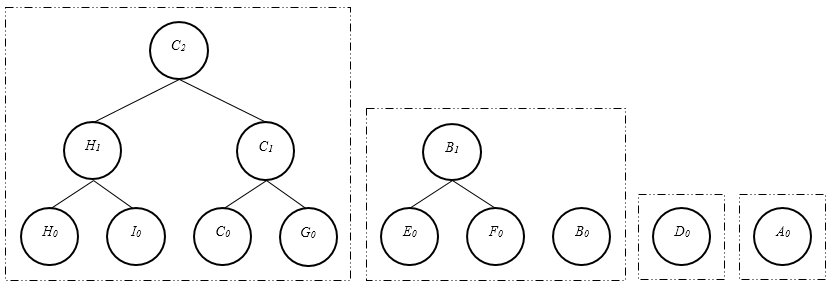
\includegraphics[width=6in]{images/commitment-tree-example-1.png}\\
					\caption{$A$ receives $C_{2}$ from $C$, $(B_{1},B_{0})$ from $B$, $D_{0}$ from $D$ and generates $A_{0}$. The commitment payload received from a given sensor node is indicated by dashed-line box.}
					\label{fig:commitment-tree-example-1}
				\end{figure}
				\begin{equation}
					\begin{array}{l}
						A_{0} = <A_{id}, 1, A_{value}, H(N||1||A_{value})>; \textsf{Sign}_{S_{A}}(A_{0}) \\
						D_{0} = <D_{id}, 1, D_{value}, H(N||1||D_{value})>; \textsf{Sign}_{S_{D}}(D_{0})\\
						B_{0} = <B_{id}, 1, B_{value}, H(N||1||B_{value})>; \textsf{Sign}_{S_{B}}(B_{0})\\
						B_{1} = <B_{id}, 2, B_{value}, H(N||2||B_{value}||E_{0}||F_{0})>; \textsf{Sign}_{S_{B}}(B_{1})\\
						\textcolor{red}{\textsf{Sign}_{S_{B}}(B_{0} || B_{1}), benefits}\\
						C_{2} = <C_{id}, 4, C_{value}, H(N||4||C_{value})||H_{1}||C_{1})>; \textsf{Sign}_{S_{C}}(C_{2})\\
						\end{array}
				\end{equation}

				\begin{figure}[h!]
					\centering
					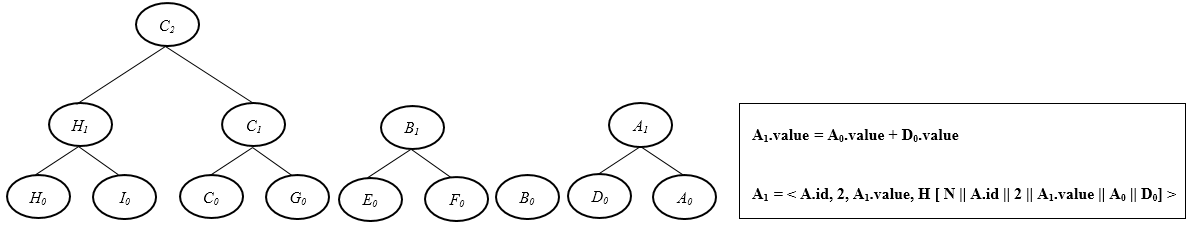
\includegraphics[width=6in]{images/commitment-tree-example-2.png}\\
					\caption{First Merge: $A_{1}$ vertex created by A.}
					\label{fig:commitment-tree-example-2}
				\end{figure}

				\begin{equation}
					\begin{array}{l}
				A_{1} = <A_{id}, 2, A_{1value}, H(N||2||A_{1value}||A_{0}||D_{0})>; \textsf{Sign}_{S_{A}}(A_{1})\\
				where\  A_{1value} = A_{value} + D_{value} \\
					\end{array}	
				\end{equation}
				\begin{figure}[h!]
					\centering
					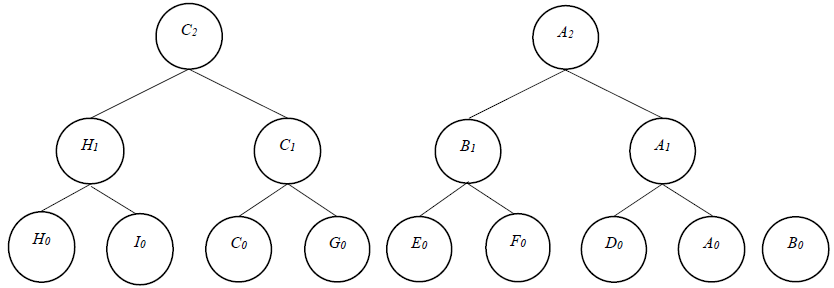
\includegraphics[width=\textwidth]{images/commitment-tree-example-3.png}\\
					\caption{Second Merge: $A_{2}$ vertex created by A.}
					\label{fig:commitment-tree-example-3}
				\end{figure}
				\begin{equation}
					\begin{array}{l}
						A_{2} = <A_{id}, 4, A_{2value}, H(N||4||A_{2value}||B_{1}||A_{1}) >; \textsf{Sign}_{S_{A}}(A_{2})\\
						where\  A_{2value} = B_{1value} + A_{1value} \\
					\end{array}
				\end{equation}
				\begin{figure}[h!]
					\centering
					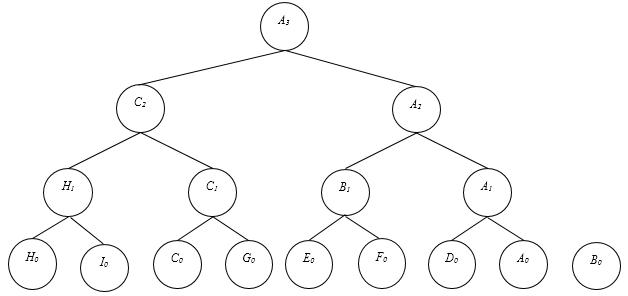
\includegraphics[width=6in]{images/commitment-tree-example-4.png}\\
					\caption{Third Merge: $A_{3}$ vertex created by A.}
					\label{fig:commitment-tree-example-4}
				\end{figure}
				\begin{equation}
					\begin{array}{l}
						A_{3} = <A_{id},8, A_{3value},H(N||8||A_{3value}||C_{2}||A_{2})>; \textsf{Sign}_{S_{A}}(A_{3})\\
						where\ A_{3value} = A_{2value} + C_{2value}
					\end{array}
				\end{equation}
			\end{exmp}
% chapter A Protocol for Commitment Tree Generation (end)

% Talk about the certificates:
	
% 	How many certificates does $A$ need to know in this example ?
% 	In the above example, $A$ need to know $D,B,C's$ certificate to verify their signatures.
% 	But if we use SHIA'a approach of creating commitment tree then $A$ need to know $E's$ certificate as well.
% 	Hence, being root in as many tree as possible is the more efficient.
\section{Bandwidth Analysis}
	For any given sensor node's forest with $n$ leaf vertices, has at most $\log n$ data-items in its payload.
	It has at most $(\log n) +1$ signatures in its payload.
	The highest possible count value is $\log n$, as all the trees are binary. 

	An intermediate sensor node $S$ with $\beta$ descendants in the aggregation tree, has at most $\log(\beta+1)$ data-items with their respective $\log(\beta+1)$ signatures in its payload.
	$S$ might need to send its payload signature $Sign(S_{p})$.
	At max, $S$ has to send a payload with $\log(\beta+1)$ data-items and $\log(\beta+1) +1$ signatures to its parent in the aggregation tree.
	
	Hence, sending signatures of the data-items causes $O(\log \beta)$ bandwidth overhead for each node in the network, where $\beta$ is the number of descendants of the sensor node. 
\section{Result checking}

\section{Performance Analysis}
	In addition to calculating its own data-items, all intermediate sensor nodes with $\beta$ descendants and $\zeta$ direct children need to do the following:
	\begin{itemize}
		\item To calculate and verify $O(\log \beta)$ signatures, creating $O(\log \beta)$ calculation overhead. 
		\item Needs sufficient memory to cache $O(\log \beta)$ certificates. 
		\item Needs enough memory to cache $\Omega(\zeta)$ certificates.
	\end{itemize}

	% Computation cost: Needs to calculate that many signatures. Needs to verify that many signatures.
	% Need to know that many certificates.

\section{Applications}
		The signature based aggregation scheme can be applied to do the \textbf{voting} in the network.
		And voting scheme can be used to solve many sensor network problems.
		For example, voting can be used to design the distributed algorithm for selecting a cluster head or node revocation system.
		In the voting scheme, following are the major security concerns: 
		\begin{itemize}
			\item The aggregate node needs to know that the vote is coming from the legit voter, no other voter is impersonating the vote of the legit voter.
			\item Only the intended aggregate node should be able to verify the vote.
			\item The aggregate node should not be able to tamper with the votes. 
			\item The aggregate node needs the proof that it aggregated the verified votes.
			\item The voter need the proof for which vote it sent to its aggregator.
		\end{itemize}
		For example, the base station wants to know the overall vote-count in the network.
		To do so, all the leaf nodes send their votes and the signature of their votes to their respective aggregate nodes in the network.
		The aggregate nodes receive votes with their signatures from all of their children voters.
		The aggregate nodes verify all the votes and count those votes.
		Then they forward the count and the signature of that count signed by the aggregate node to their respective parent in the aggregation tree.
		This process is repeated until the final count and its signature, is sent to the base station by the root of the aggregation tree.
				
	\textbf{Node power level},
	\textbf{Surveillance Application}
